\documentclass[12pt]{report}

\usepackage[a4paper,width=150mm,top=25mm,bottom=25mm,bindingoffset=6mm]{geometry}
\usepackage[onehalfspacing]{setspace}
\usepackage{ucs}
\usepackage[table,xcdraw]{xcolor}
\definecolor{mColor1}{rgb}{0.9,0.9,0.9}

\usepackage{fancyhdr}
\pagestyle{fancy}
\fancyhead{}
\renewcommand{\chaptermark}[1]{\markboth{#1}{}}
\renewcommand\sectionmark[1]{\markright{\thesection\ #1}}

\fancyhead[LO, RE]{\leftmark}
\fancyhead[LE, RO]{\rightmark}

\usepackage{titlesec, blindtext, color}
\definecolor{gray75}{gray}{0.75}
\usepackage{mathptmx}
\usepackage[utf8]{inputenc}
\usepackage[T1]{fontenc}
\usepackage[ngerman]{babel}

\usepackage{amsmath,amssymb,amstext,amsthm,mathtools}
\usepackage{url}
\usepackage{caption}
%\usepackage[belowskip=-5pt,aboveskip=0pt]{caption}
\usepackage{subcaption}

\usepackage{float}
\usepackage{lscape}
\usepackage{pdfpages}
\usepackage{rotating}
\usepackage{graphicx}
\setlength\parindent{0pt}
\usepackage{hyperref}
\usepackage{acronym}
\usepackage{textcmds}
\usepackage{longtable}
\usepackage[export]{adjustbox}
\usepackage{upgreek}
\usepackage{dsfont}
\usepackage{tensor}
\usepackage{amsbsy}
\usepackage{multirow, hhline, colortbl}
\usepackage[table]{xcolor}


\DeclareMathAlphabet{\mathcal}{OMS}{cmsy}{m}{n}
\SetMathAlphabet{\mathcal}{bold}{OMS}{cmsy}{b}{n}

\usepackage{listings, lstautogobble}
\usepackage{textcomp}
\definecolor{yo}{rgb}{0.9,0.6,0}
\definecolor{Gray}{gray}{0.9}
\definecolor{listinggray}{gray}{0.9}
\definecolor{lbcolor}{rgb}{0.95,0.95,0.95}
\definecolor{greylines}{rgb}{0.9529,0.9529,0.9529}

\lstset{
	backgroundcolor=\color{lbcolor},
	tabsize=4,
	rulecolor=,
	language=python,
        basicstyle=\scriptsize,
        upquote=true,
        aboveskip={1.5\baselineskip},
        columns=fixed,
        showstringspaces=false,
        extendedchars=true,
        breaklines=true,
        prebreak = \raisebox{0ex}[0ex][0ex]{\ensuremath{\hookleftarrow}},
        frame=lines,
        showtabs=false,
        showspaces=false,
        showstringspaces=false,
        identifierstyle=\ttfamily,
        keywordstyle=\color[rgb]{0.55,0,0},
        alsoletter={/,*,[,]},%
        otherkeywords={},
        morekeywords=[2]{with, as},
        morekeywords=[3]{},
        emph={self},          % Custom highlighting
		emphstyle=\color[rgb]{0.1,0.3,1},
		emph={[2]f},          % Custom highlighting
		emphstyle={[2]\color[rgb]{0.1,0.5,0.1}},
		emph={[3]__init__},          % Custom highlighting
		emphstyle={[3]\color[rgb]{0.1,0.3,1}},
		emph={[4]open,str,print,KeyError},          % Custom highlighting
		emphstyle={[4]\color[rgb]{0.2,0.6,0.8}},
        commentstyle=\color[rgb]{0.3,0.3,0.3},
        stringstyle=\color[rgb]{0.133,0.545,0.133},
        	autogobble=true
}
\lstnewenvironment{ttlisting}{\lstset{basicstyle=\scriptsize}}{}

\usepackage{color}
\usepackage[section]{placeins}

\newenvironment{simplechar}{%
	\catcode`\$=12
	\catcode`\&=12
	\catcode`\#=12
	\catcode`\^=12
	\catcode`\_=12
	\catcode`\~=12
	\catcode`\%=12
	\catcode`\"=12
	\catcode`\'=12
	}{}{}

\newtheoremstyle{dotless}{}{}{\itshape}{}{\bfseries}{}{ }{}

\theoremstyle{dotless}

\newtheorem{thm}{Theorem}
\newtheorem{defn}[thm]{Definition}
\newtheorem{exmp}[thm]{Example}
\theoremstyle{definition}


\begin{document}

\begin{titlepage}
	Warum bin ich nicht einfach Staubsaugervertreter geworden?
\end{titlepage}

\tableofcontents

\chapter{Reservierungsprozess und seine Schnittstellen}

\section{Aktuar in der Schadenversicherung}

\subsection{Kernaufgaben und Funktionen}

\begin{itemize}
	\item Bewertung von R�ckstellungen f\"ur Sch\"aden, Pr\"amien, Regulierungskosten und Regresse
	\item Tarifierung und Produktentwicklung
	\item Risikomanagement
	\item Controlling
	\item Aufsichtsrechtliche und regulatorische Funktionen
	\item[$\rightarrow$] Methodenstetigkeit und Datenstetigkeit zu beachten
\end{itemize}

\subsection{Zielsetzungen Reservebewertung}
\begin{itemize}
	\item Bestimmung der R\"uckstellungen f\"ur bilanzielle Zwecke
	\item Unternehmensanalyse durch Ratingagentur
	\item Shareholder-Value-Betrachtung
	\item Ermittlung angemessener Pr\"amien
\end{itemize}

\subsubsection{Reservierungsprozess}

\begin{figure}[H]
\centering
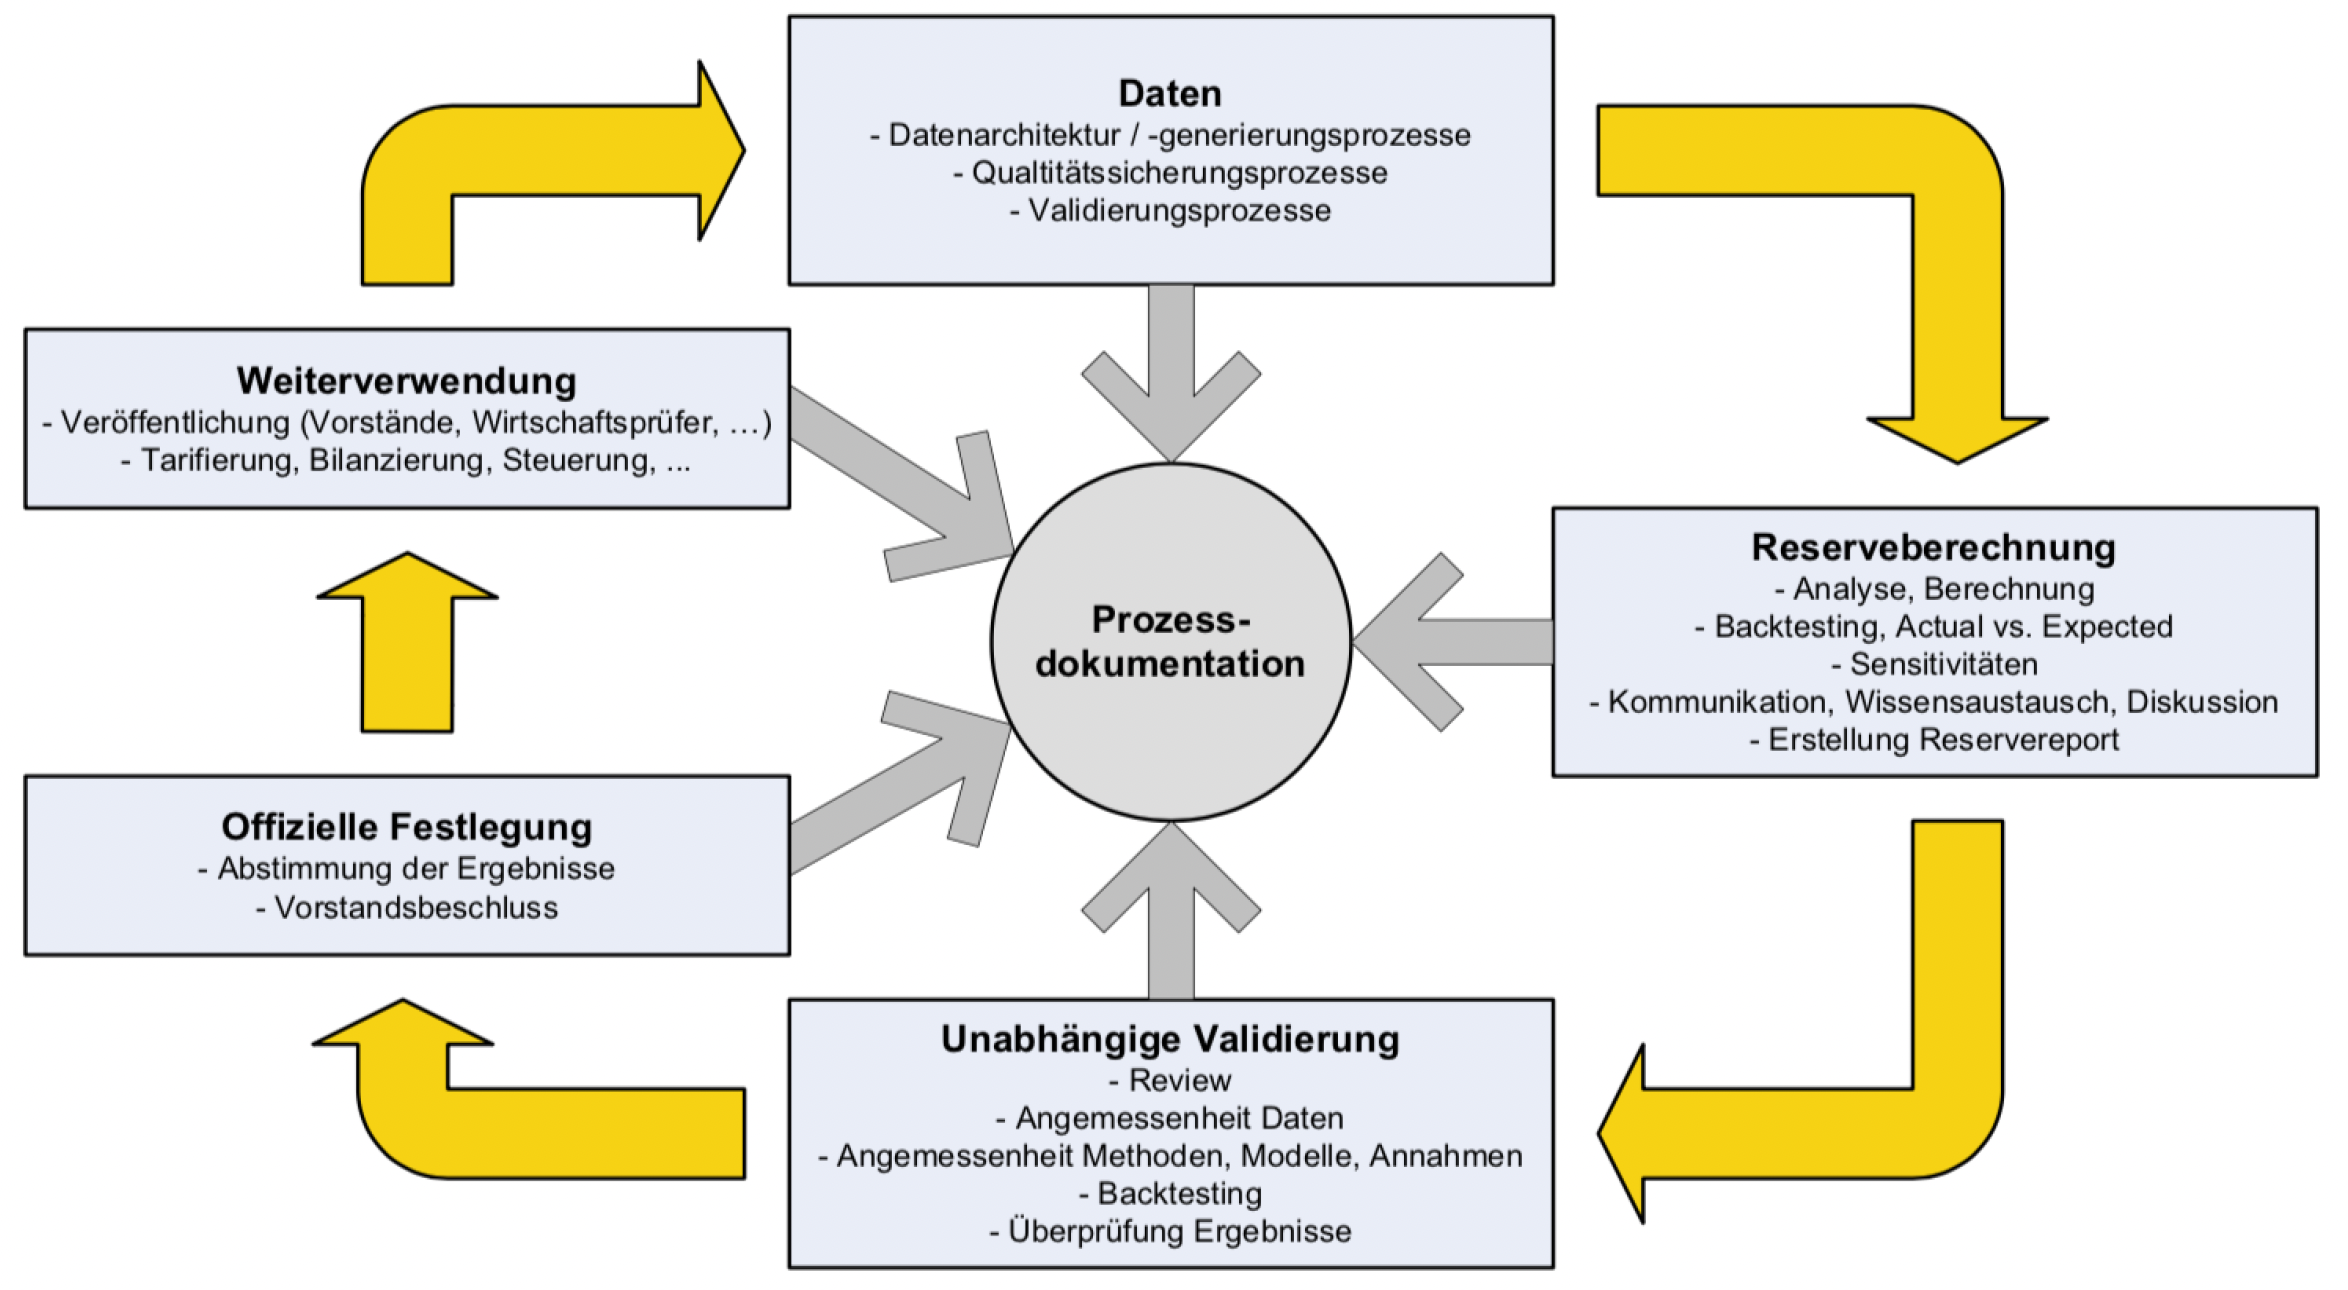
\includegraphics[width=\textwidth]{Bilder/Reservierungsprozess.png}
\end{figure}


\subsubsection{Allgemeine Aspekte}
\begin{itemize}
	\item Umfang und Turnus
	\item Rollenbeschreibung der Beteiligten
	\item Organisationsstruktur
	\item Unabh\"angigkeit und Objektivit\"at
	\item Interne Kontrollen
\end{itemize}

\subsubsection{Daten}
\begin{itemize}
	\item Transparanz, Nachvollziehbarkeit der Datengenerierung
	\item Dokumentation des Prozesses
	\item Beschreibung Datenarchitektur
	\item unternehmensweite Konsisntenz
	\item ausreichende Datenhistorie
	\item Qualit\"atssicherung mit angemessener Dokumentation
	\item automatische und manuelle Tests
	\item Plausibilisierung
\end{itemize}

\subsubsection{Reserveberechnung}
\begin{itemize}
	\item Festlegung von Umfang der Analysen und Konsistenz zu SII
	\item Welche Software?
	\item Welche Annahmen werden wie getroffen?
	\item Wie sieht die aktuarielle Entscheidungsfindung aus und ist diese transparent dokumentiert?
	\item Wie wird kontrolliert und validiert?
\end{itemize}

\subsubsection{Unabh\"angige Validierung}
\begin{itemize}
	\item insb. durch SII gefordert
	\item \"Uberpr\"ufung der Angemessenheit der Daten, Modelle, Methoden, Annahmen und Ergebnisse
	\item Backtesting
	\item unabh\"angig von der Berechnung
\end{itemize}

\subsubsection{Prozessdokumentation}
\begin{itemize}
	\item Prozessbeschreibung
		\begin{itemize}
			\item �berblick
			\item Schnittstellen
			\item Prozessgestaltung
			\item Ausf\"uhrung
			\item Versionshistorie
			\item Kontrollsystem
			\item Tests
			\item Dokumentationsrichtlinien
		\end{itemize}
	\item Dokumentation der Kontrollprozesse
\end{itemize}

\subsection{Zweck und Aufbau des Reserveberichts}
\begin{itemize}
	\item Reservebericht 
	\begin{itemize} 
		\item individuell an Umfang und Verwendungszweck angepasst
		\item an Zielgruppen orientiert
		\item als Basis der VmF zur Erf�llung ihrer Pflichten
	\end{itemize}
	\item Inhalte des Reserveberichts
	\begin{itemize}
		\item Zweck der Reserveanalyse, Auftraggeber
		\item Umfang der Reserveanalyse
		\item Relevante Entwicklungen und wesentliche Kennzahlen
		\item Daten und Methoden
		\item Zusammenfassung der Ergebnisse
		\item Vergleich mit Vorperioden
	\end{itemize}
\end{itemize}

\chapter{Versicherungstechnische R�ckstellungen in der Rechnungslegung}

\section{IFRS 17, HGB, SII im Vergleich}

Unterschieden wird nach:
\begin{itemize}
	\item IFRS 17: entscheidungsn\"utzliche Informationen bzgl. Verm\"ogens- und Finanzlage
	\item HGB: Informationsvermittlung und Aussch\"uttungsbemessung
	\item SII: Bestimmung der Eigenmittel als Verlustdeckungspotenzial 
\end{itemize}

\subsection{Versicherungsvertr\"age}

\begin{itemize}
	\item IFRS 17: Vertr\"age, die signifikantes Versicherungsrisiko \"ubertragen (Versicherungsrisiko wird von Finanzrisiko abgegrenzt)
	\item HGB: keine eigene Definition von Versicherungsvertr\"agen, aber Anforderungen an den Risikotransfer von R\"uckversicherung
	\item SII: keine eigene Definition von Versicherungsvertr\"agen und R\"uckversicherungsvertr\"agen
\end{itemize}

\subsection{Kosten als Teil der vers.techn. R\"uckstellungen}

\begin{itemize}
	\item IFRS 17: SRK und Verwaltungskosten werden einbezogen, Ber\"ucksichtigung der variablen Abschlusskosten bei CSM, keine allgemeine Verwaltungskosten ber\"ucksichtigt
	\item HGB: SRK einbezogen, keine allgemeine Verwaltungskosten ber\"ucksichtigt
	\item SII: SRK, Vertragsverwaltungskosten, Abschlusskosten, Kosten der Verwaltung der Kapitalanlagen einbezogen
\end{itemize}

\subsection{Datenqualit\"at}
\begin{itemize}
	\item HGB: Grunds�tze ordnungsgem\"a{\ss}er Buchf\"uhrung
	\item SII:
	\begin{itemize}
		\item Vollst�ndigkeit, Richtigkeit und Angemessenheit gefordert
		\item bezieht sich auf interne und externe Daten
		\item Angemessenheit muss nachweisbar sein, daf\"ur umfangreiche Dokumentation erforderlich
	\end{itemize}
	\item IFRS 17: kein eigener Abschnitt zur Datenqualit\"at
\end{itemize}

\section{Bewertungsmodell unter IFRS 17}

Building Block Approach (u.U. Premium Allocation Approach zugelassen):
\begin{itemize}
	\item Basis sind die erwarteten Zahlungsstr�me
	\item Diskontierung
	\item Risikomarge zur Deckung der Unsicherheiten (keine Berechnungsvorgabe, aber geforderte Eigenschaften)
	\item Servicemarge (CSM) dient der Neutralisierung von Gewinnen bei Vertragsabschluss. Bei LIC (Liability for incurred claims keine CSM)
	\item LRC (Liability for remaining coverage) f�r bound but not incepted onerous contracts wird eine Drohverlustr\"uckstellung (Loss Component) gebildet, f\"ur incepted contracts eine CSM
\end{itemize}

\section{Bewertungsmodell unter HGB}
Retrospektive Bewertung der Beitr\"age mit prospektiver Bildung von R"uckstellungen f\"ur drohende Verluste. Bewertung der Schadenr\"uckstellung prospektiv:
\begin{itemize}
	\item Einzelbewertung f\"ur bekannte Versicherungsf\"alle
	\item Gruppenbewertung f\"ur unbekannte Sp\"atsch\"aden
	\item Rentenverbindlichkeiten separat bewerten
	\item Zus\"atzliche Schwankungsr\"uckstellungen zur Stabilisierung
\end{itemize}

\subsection{Schwankungsr\"uckstellungen unter HGB}
	\begin{itemize}
		\item zu bilden, wenn erhebliche Schwankungen erwartet werden oder Schwankungen nicht durch Beitr\"age ausgeglichen werden k\"onnen oder durch R\"uckversicherung gedeckt sind
		\item Nur bei Schaden/Unfall
		\item Ermittlung und Bildung f\"ur jeden Versicherungszweig separat.
		\item Berechnung Standardfall:
		\begin{itemize}
			\item $\{1,...,n\}$ der Beobachtungszeitraum vor Bilanzjahr $n+1$
			\item $\bar{q}$ die durchschnittliche Schadenquote, $\bar{\sigma} = \sqrt{\frac{1}{n-1}\sum^{n}_{i=1}(q_i-\bar{q})^2}$ die Standardabweichung
			\item Sollbetrag $SB=4,5 \cdot \bar{\sigma} \cdot P$, $P \hat{=}$ verdiente Beitr\"age des Bilanzjahres
			\item[(1)] $SR^{(1)}_{n+1} = \begin{cases}
				min(SR_n + 3,5\% \cdot SB; SB) & \text{falls } SR_n \leq SB \\
				SR_n & \text{sonst}
			\end{cases}$ 
			\item $B=(\bar{q} - q_{n+1}) \cdot P$ ,\ ($\bar{q} > q_{n+1} \rightarrow$ B Unterschaden, $\bar{q} < q_{n+1} \rightarrow$ -B \"Uberschaden)
			\item[(2)] Erh\"ohung bei Unterschaden: \\ $SR^{(2)}_{n+1} = \begin{cases}
				min(SR_{n+1}^{(1)} + B; SB) & \text{falls } SR_{n+1}^{(1)} \leq SB \text{ und } \bar{q} > q_{n+1}\\
				SR_n	{(1)} & \text{sonst}
			\end{cases}$  
			\item[(3)] Entnahme des \"Uberschadens: \\
			$SR^{(3)}_{n+1} = \begin{cases}
				max(SR_{n+1}^{(2)} + B; 0) & \text{falls } \bar{q} < q_{n+1}\\
				SR_{n+1}^{(2)} & \text{sonst}
			\end{cases}$ 
			\item[(4)] Begrenzung durch Sollbetrag sicherstellen \\
			$SR_{n+1} = min(SR_{n+1}^{(3)}; SB)$
			\item Schadenquote nach Schwankung: $q_{n+1}^{nS} = q_{n+1} + \frac{SR_{n+1} - SR_n}{P}$
			\item Falls $SR_{n+1} = SR_n + 3,5\% \cdot SB + B$, dann $q_{n+1}^{nS} = \bar{q} + 3,5\% \cdot 4,5 \cdot \bar{\sigma}$
		\end{itemize}
			
	\end{itemize}

\subsection{Bewertungsmodell unter SII}

\begin{itemize}
	\item prospektive Bewertung des gesamten Versicherungsvertrags:
	\begin{itemize}
		\item Basis: erwartete Zahlungsstr\"ome
		\item risikolose Diskontierung
		\item Risikomarge
	\end{itemize}
	\item vers.techn. R\"uckstellungen (TPs) beinhalten Claims Provisions, Premium Provisions (beides diskontiert) und Risikomarge
	\item BE einer vers.techn. R\"uckstellung $\hat{=}$ wahrscheinlichkeitsgewichteter Durchschnitt zuk\"unftiger Zahlungensstr\"ome unter Ber\"ucksichtigung des Zeitwerts des Geldes (Barwert) und unter Verwendung einer risikofreien Zinskurve (existiert brutto und netto) 
\end{itemize}

\subsection{Schadenr\"uckstellungen unter SII}

\begin{itemize}
	\item Schadenr\"uckstellungen decken die Verpflichtungen aus bereits eingetretenen Sch\"aden zu Vertr\"agen, die vor dem Bilanzstuchtag bestanden haben inkl. noch unbekannter Rentenf\"alle
	\item BE einer Schadenr\"uckstellung $\hat{=}$ diskontierter wahrscheinlichkeitsgewichteter Durchschnitt k�nftiger Sch\"aden, die sich vor dem Bilanzstichtag ereignet haben
	\item Zuk\"unftige Zahlungsstr\"ome der SRK sind Teil der Schadenr\"uckstellungen
\end{itemize}

\subsection{Pr\"amienr\"uckstellungen unter SII}

\begin{itemize}
	\item Pr\"amienr\"uckstellungen $\hat{=}$ Saldo aus Barwert der Verpflichtungen und Barwert zuk\"unftiger Pr\"amien
	\item Barwert der Verpflichtungen bezieht sich auf zuk\"unftig eintretende Schadenf\"alle aus Vertr\"agen, die zum Bilanzstichtag bestanden haben
\end{itemize}

\subsubsection{Ansatz von Versicherungsvertr\"agen unter SII}
\begin{itemize}
	\item Bei Berechnung der Pr\"amienr\"uckstellungen sind alle Zahlungsstr\"ome zu ber\"ucksichtigen
	\item Entscheidend ist ob Beginn des Versicherungsschutzes oder der Vertragsabschluss vor Bilanzstichtag liegt
\end{itemize}

\subsubsection{Vertragsgrenzen unter SII}
\begin{itemize}
	\item Anzusetzende Vertr\"age sind bis zum folgenden Zeitpunkt in der Berechnung der Pr\"amienr\"uckstellungen zu ber\"ucksichtigen:
	\begin{itemize}
		\item bis zu dem Tag, an dem das Versicherungsunternehmen das einseitige Recht hat, den Vertrag zu beenden
		\item bis zu dem Tag, an dem das Versicherungsunternehmen das einseitige Recht hat, die Pr\"amienh\"ohe oder den Leistungsumfang anzupassen
	\end{itemize}	
\end{itemize}

\subsubsection{Vereinfachtes Berechnungsverfahren zur Sch\"atzung der Pr\"amienr\"uckstellung}

\begin{itemize}
	\item undiskontierte Pr\"amienr\"ucktellungen \begin{equation}
		BE_{premium} = (CR - AER) \cdot VM + (CR - 1) \cdot FP
	\end{equation} 
	\item CR: gesch\"atzte, undiskontierte Schaden-Kosten-Quote
	\item AER: gesch\"atzte Abschlusskostenqote f\"ur Abschlusskosten des aktuellen Bestandes, die bis zum Laufzeitende angefallen sind
	\item VM: \"okonomische Beitrags\"ubertr\"age aus bereits bekannten Vertr\"agen
	\item FP: gesch\"atzte, zuk\"unftige, undiskontierte Brutto-Pr\"amie f\"ur alle Vertr\"age des aktuellen Bestandes, die gem\"a{\ss} der Grenzen der Versicherungsvertr\"age zu ber\"ucksichtigen sind
 \end{itemize}


















\end{document}
